\documentclass[handout, 10pt]{beamer}

%\usepackage[backend=bibtex,firstinits=true,style=verbose-inote,citestyle=authortitle]{biblatex}
\usepackage{bm}
\usepackage{graphicx}
\usepackage{subcaption}
\usepackage{amsmath}
\usepackage{amsfonts}
\usepackage{makecell}
\usepackage{filecontents}
\usepackage{biblatex}
\usepackage{xcolor}
\usepackage{subcaption}
% \newcommand{\expect}[2][]{
\ifthenelse{\equal{#1}{}}{
\mathbb{E}\left[#2\right]
}{
\underset{#1}{\mathbb{E}}\left[#2\right]
}}

\newcommand{\cov}[2][]{
\ifthenelse{\equal{#1}{}}{
\text{Cov}\left[#2\right]
}{
\underset{#1}{\text{Cov}}\left[#2\right]
}}


\newcommand{\var}[2][]{
\ifthenelse{\equal{#1}{}}{
\text{Var}[#2]
}{
\underset{#1}{\text{Var}}[#2]
}}

\newcommand{\loss}[2][]{
\ifthenelse{\equal{#1}{}}{
\mathcal{L}(#2)
}{
\mathcal{L}_{#1}(#2)
}}

\newcommand{\kl}[2]{
\text{D}_\text{KL}[#1 \parallel #2]
}

\newcommand{\R}{\mathbb{R}}
%\newcommand{\Prob}{\mathbb{P}}

\newcommand{\1}[1]{\mathds{1}\{#1\}}


%\usecolortheme{dolphin}
\setbeamertemplate{navigation symbols}{}
\setbeamertemplate{section in toc}{\inserttocsectionnumber.~\inserttocsection}

\begin{filecontents*}{references.bib}
@InProceedings{StyleGAN2,
author = {Karras, Tero and Laine, Samuli and Aittala, Miika and Hellsten, Janne and Lehtinen, Jaakko and Aila, Timo},
title = {Analyzing and Improving the Image Quality of StyleGAN},
booktitle = {Proceedings of the IEEE/CVF Conference on Computer Vision and Pattern Recognition (CVPR)},
month = {June},
year = {2020}
}
\end{filecontents*}

\addbibresource{references.bib}


\title{Analyzing and Improving the Image Quality of StyleGAN\footnote{\citepaper{StyleGAN2}}}
%\subtitle{}
%\author{Ivan Skorokhodov}
%\date{}
%\logo{\includegraphics[height=1cm]{images/ipavlov-logo.png}}

\newcommand{\citepaper}[1]{\citetitle{#1} by \citeauthor{#1}, \citeyear{#1}}

%\graphicspath{{./images}}

%\usetheme{lucid}
\begin{document}

\begin{frame}
    \titlepage
\end{frame}

\begin{frame}{Overview}
\begin{itemize}
    \item\pause Authors improve several flaws of StyleGAN2
    \begin{itemize}
        \item\pause Remove \textit{droplet artifacts} by replacing AdaIN
        \item\pause Remove \textit{phase artifacts} by replacing progressive growing with multi-scale gradients
        \item\pause Make latent space nicer by introducing \textit{path length regularization}
    \end{itemize}
    \item\pause Overall, scores are improved by up to 30\% in terms of quantitative metrics
\end{itemize}

\end{frame}


\begin{frame}{StyleGAN architecture}
\begin{columns}
 \begin{column}{.49\textwidth}
    \begin{figure}
        \centering
        \includegraphics[width=\textwidth]{images/stylegan-architecture}
    \end{figure}
 \end{column}

\begin{column}{.49\textwidth}
\begin{itemize}
    \small
    \item\pause Two sources of noise: latent noise $z$ and many additional channel-wise noises at each resolution
    \item\pause $z$ is transformed into latent code $w$ through a mapping network
    \item\pause Latent vector $w$ is passed through AdaIN layers
    \item\pause Uses progressive growing
\end{itemize}
 \end{column}
\end{columns}
\end{frame}


\begin{frame}{Adaptive Instance Normalization (AdaIN)}
\begin{itemize}
    \item\pause AdaIN is similar to batch normalization, but operates on an instance-wise basis
    \item\pause It replaces statistics $\mu_i(x_i), \sigma_i(x_i)$ of filter map $x_i$ with the externally provided ones $y_{b,i}, y_{s,i}$:
\begin{equation}
\operatorname{AdalN}\left(\mathbf{x}_{i}, y_{b,i}, y_{s,i}\right)=\mathbf{y}_{s, i} \frac{\mathbf{x}_{i}-\mu\left(\mathbf{x}_{i}\right)}{\sigma\left(\mathbf{x}_{i}\right)}+\mathbf{y}_{b, i}
\end{equation}
    \item\pause StyleGAN passes $w$ into $G$ via AdaIN instead of feed-forward layers as is usually done
\end{itemize}
\end{frame}


\begin{frame}{Droplet artifact}
AdaIN causes droplet artifacts:
\begin{figure}
\centering
\includegraphics[width=\textwidth]{images/droplet-artifact}
\end{figure}
\begin{itemize}
    \item\pause Imagine that $G$ carries some important information in activations magnitudes
    \item\pause Generally, normalization procedure erases this information
    \item\pause A dirty workaround for $G$ to preent the erasion is to make some activations \textit{huge}
    \item\pause This allows it to set mean/std for the remaining activations to the desired value
\end{itemize}
\end{frame}


\begin{frame}{Weights demodulation}
\begin{itemize}
    \item\pause Authors noticed that it is not necessary to normalize the mean
    \item\pause Then they noticed that updating the std is equivalent to rescaling convolutional weights 
\end{itemize}

\begin{figure}
\centering
\includegraphics[width=\textwidth]{images/weight-demodulation}
\end{figure}
\end{frame}


\begin{frame}{Perceptual Path Length}
StyleGANv1 paper proposed PPL metric to measure the latent space quality
\begin{equation}
\begin{aligned}
\ell_{\mathcal{Z}}=\mathbb{E}\left[\frac{1}{\epsilon^{2}} d\left(G\left(\operatorname{slerp}\left(\mathbf{z}_{1}, \mathbf{z}_{2} ; t\right)\right), G\left(\operatorname{slerp}\left(\mathbf{z}_{1}, \mathbf{z}_{2} ; t+\epsilon\right)\right)\right)\right]
\end{aligned}
\end{equation}

where $d$ is the \textit{perceptual distance}, i.e. a $L_2$ distance between VGG16 embeddings.

\end{frame}


%\begin{frame}{FYI: Spherical interpolation (slerp)}
%\begin{itemize}
%    \item\pause Since the high-dimensional gaussian distribution is concentrated on a sphere, slepr is more preferrable than the linera interpolation
%    \item\pause slerp is computed as: 
%\end{itemize}
%\end{frame}


\begin{frame}{Path length regularization}
Authors noticed that PPL correlates very well with image quality and propose a way to optimize it during training:
\begin{equation}
\mathbb{E}_{\mathbf{w}, \mathbf{y} \sim \mathcal{N}(0, \mathbf{I})}\left(\left\|\mathbf{J}_{\mathbf{w}}^{T} \mathbf{y}\right\|_{2}-a\right)^{2}
\end{equation}
where:
\begin{itemize}
    \item $J_w$ is the Jacobian of $G$ with respect to latent code $\bm w$
    \item $\bm y$ is a random image of size $512\times 512 \times 3$
    \item $a$ is computed as EMA of $\|\mathbf{J}_{\mathbf{w}}^{T} \mathbf{y}\|_{2}$
    \item\pause The motivation is to make $G$ change its output by a constant value when $w$ is changed by a constant value
    \item\pause They prove that it is minimized when $J_w$ is orthogonal
    \begin{itemize}
        \item\pause i.e. output is changing at the same speed as the input
    \end{itemize}
\end{itemize}
\end{frame}

\begin{frame}{Progressive growing}
ProGAN gently adds new layers during training increasing the resolution:
\begin{figure}
\centering
\includegraphics[width=\textwidth]{images/progressive-growing}
\end{figure}

\pause
After adding a layer we use a weighted sum for a new output resolution:
\begin{equation}
x_\text{out} = \alpha \cdot x_\text{new} + (1 - \alpha) \cdot \text{upsample}(x_\text{old})
\end{equation}
and $\alpha$ is gradually increased from 0 to 1.
\end{frame}

\begin{frame}{Phase artifact}
\begin{figure}
\centering
\includegraphics[width=0.7\textwidth]{images/phase-artifact}
\end{figure}
\begin{itemize}\small
    \item\pause We rotate a face, but teeth are not rotated
    \item\pause Authors blame progressive growing for this:
    \begin{itemize}
        \item\pause During training, $x_\text{old}$ is used to produce an image of twice higher resolution than it is suitable for
        \item\pause This forces $G$ to generate excessively high frequencies for lower resolutions
        \item\pause This forces $G$ to decide on important details too early during a forward pass
        \item\pause This ``compromises shift invariance''\footnote{I didn't get that too.}
    \end{itemize}
\end{itemize}
\end{frame}

\begin{frame}{Multi-scale gradient}
\begin{figure}
\centering
\includegraphics[width=\textwidth]{images/msg}
\end{figure}

Authors incorporate MSG in StyleGAN2 and remove progressing growing.\footnote{They modify it a lot but it's out of scope}
\end{frame}


\begin{frame}{Lazy regularization}
\begin{itemize}
    \item\pause Instead of WGAN-GP penalty, they use R1-penalty:
\begin{equation}
R_{1}:=\frac{\gamma}{2} \mathrm{E}_{p_{\mathcal{D}}(x)}\left[\left\|\nabla D(x)\right\|^{2}\right]
\end{equation}
    \item\pause They compute it only once in 16 iterations which makes training faster
    \item\pause They also compute PLR regularization once in 8 iterations
    \item\pause This requires tweaking Adam optimizer
\end{itemize}
\end{frame}



\begin{frame}{Final scores}
\begin{figure}
\centering
\includegraphics[width=\textwidth]{images/stylegan2-scores}
\end{figure}    
\end{frame}


\begin{frame}{Cherry-picked samples}
\begin{figure}
\centering
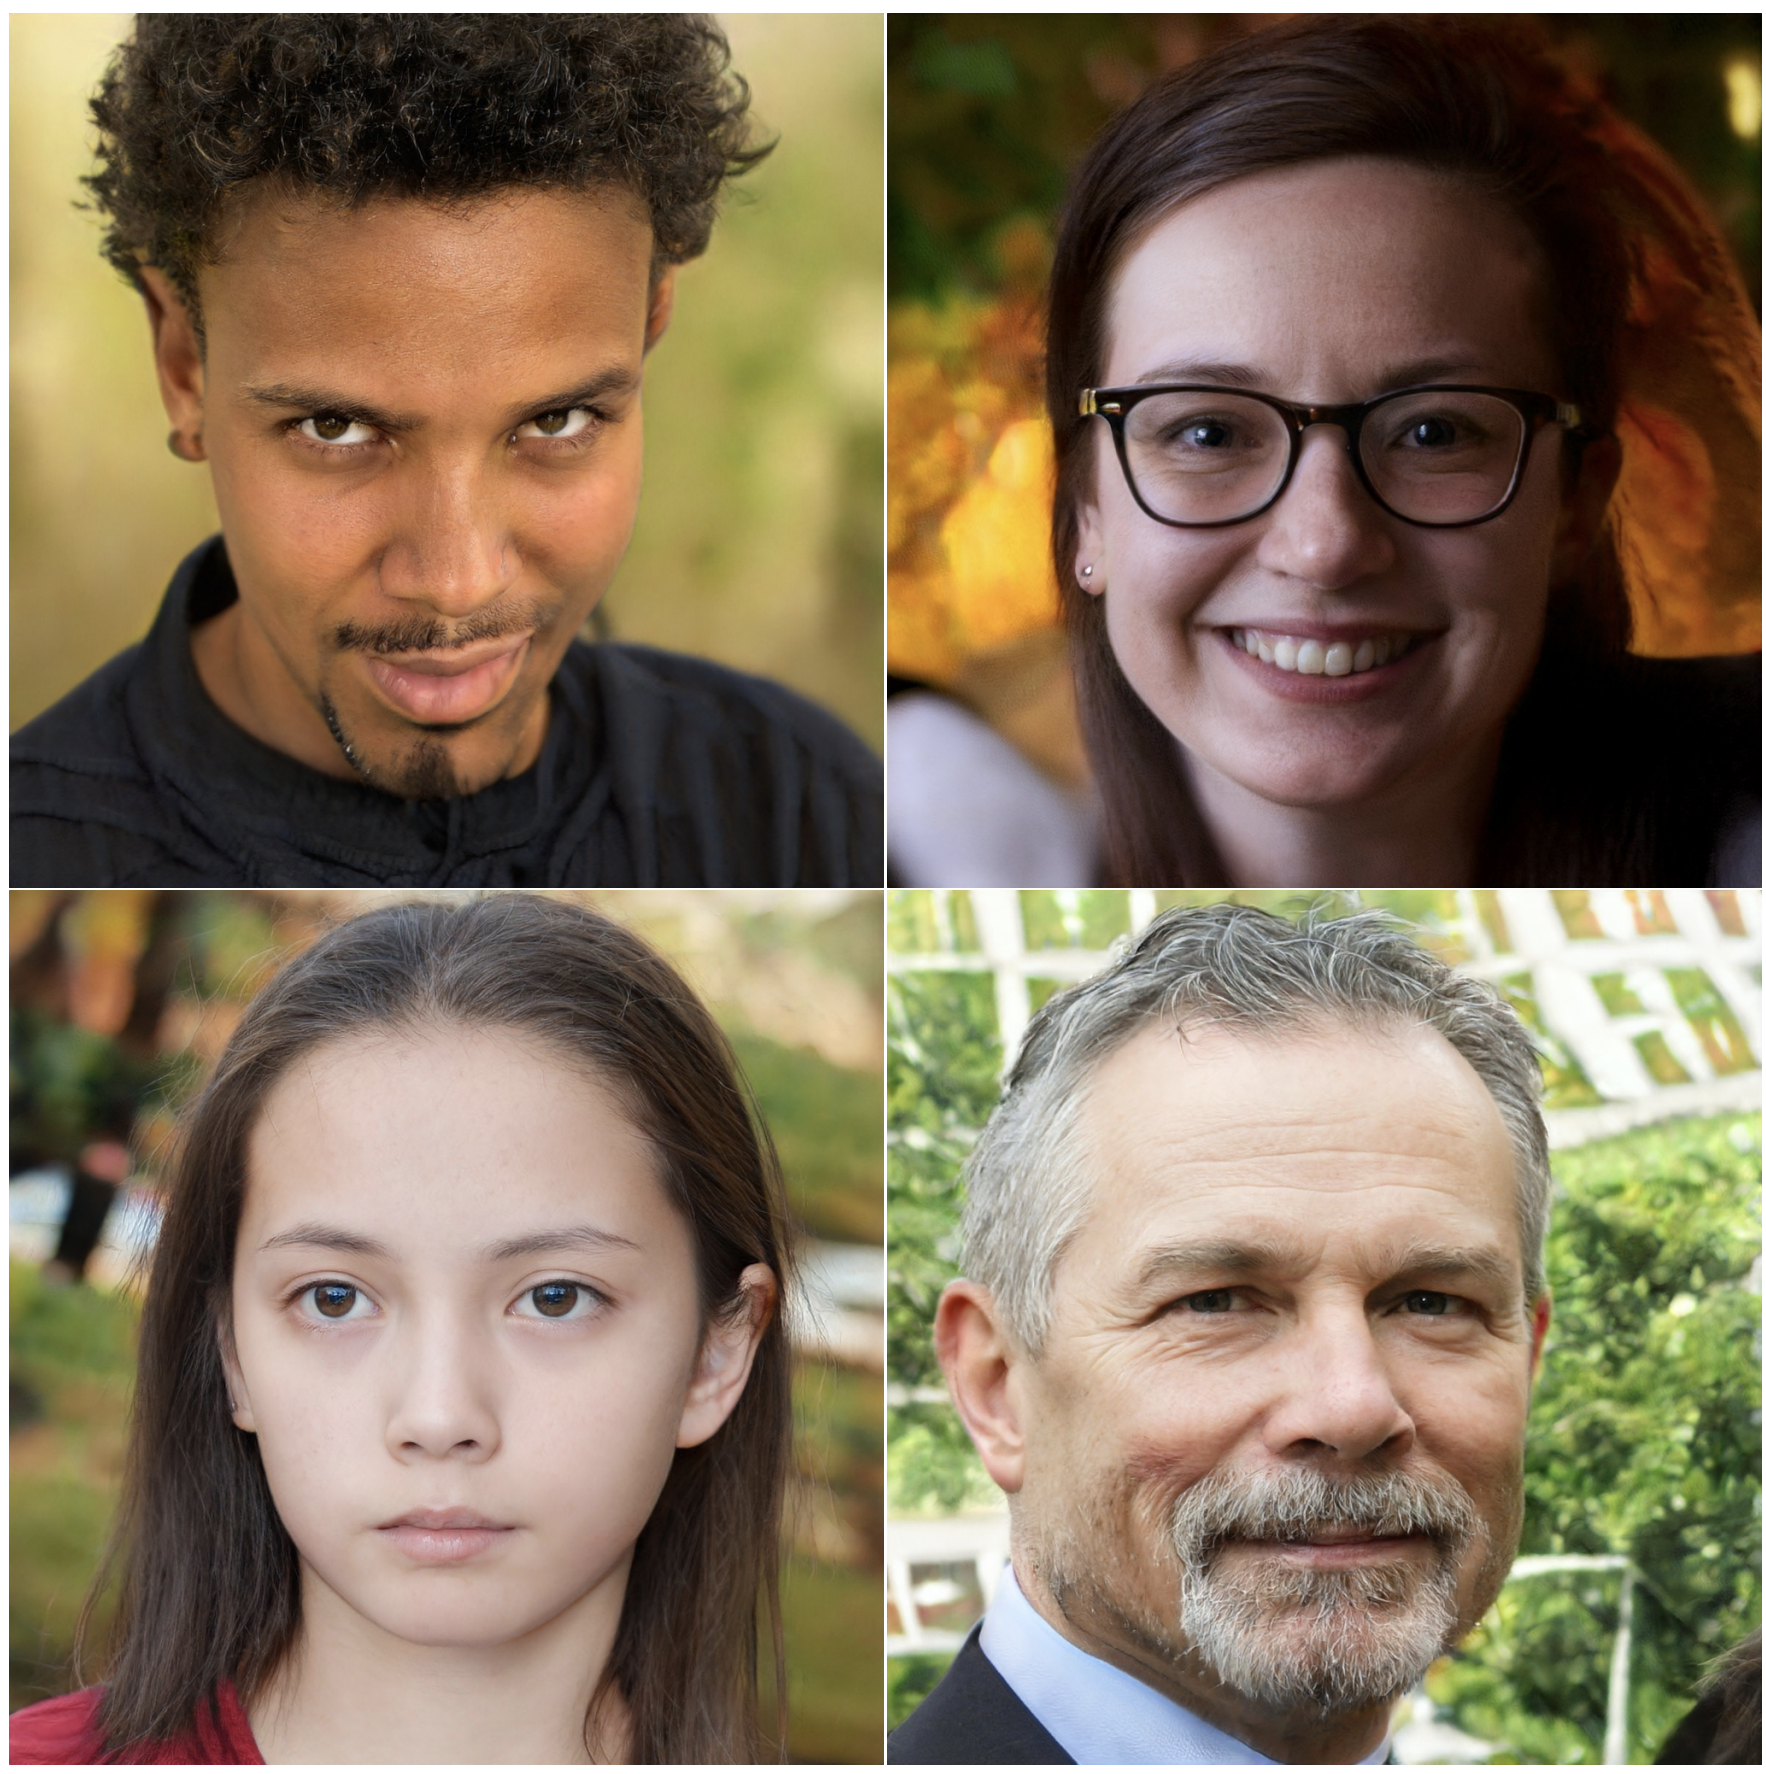
\includegraphics[width=0.7\textwidth]{images/stylegan2-cherrypicked-samples}
\end{figure}
\end{frame}


\begin{frame}{Non-cherrypicked samples 1/2}
\begin{figure}
\centering
\includegraphics[width=\textwidth]{images/stylegan2-samples-1}
\end{figure}
\end{frame}


\begin{frame}{Non-cherrypicked samples 2/2}
\begin{figure}
\centering
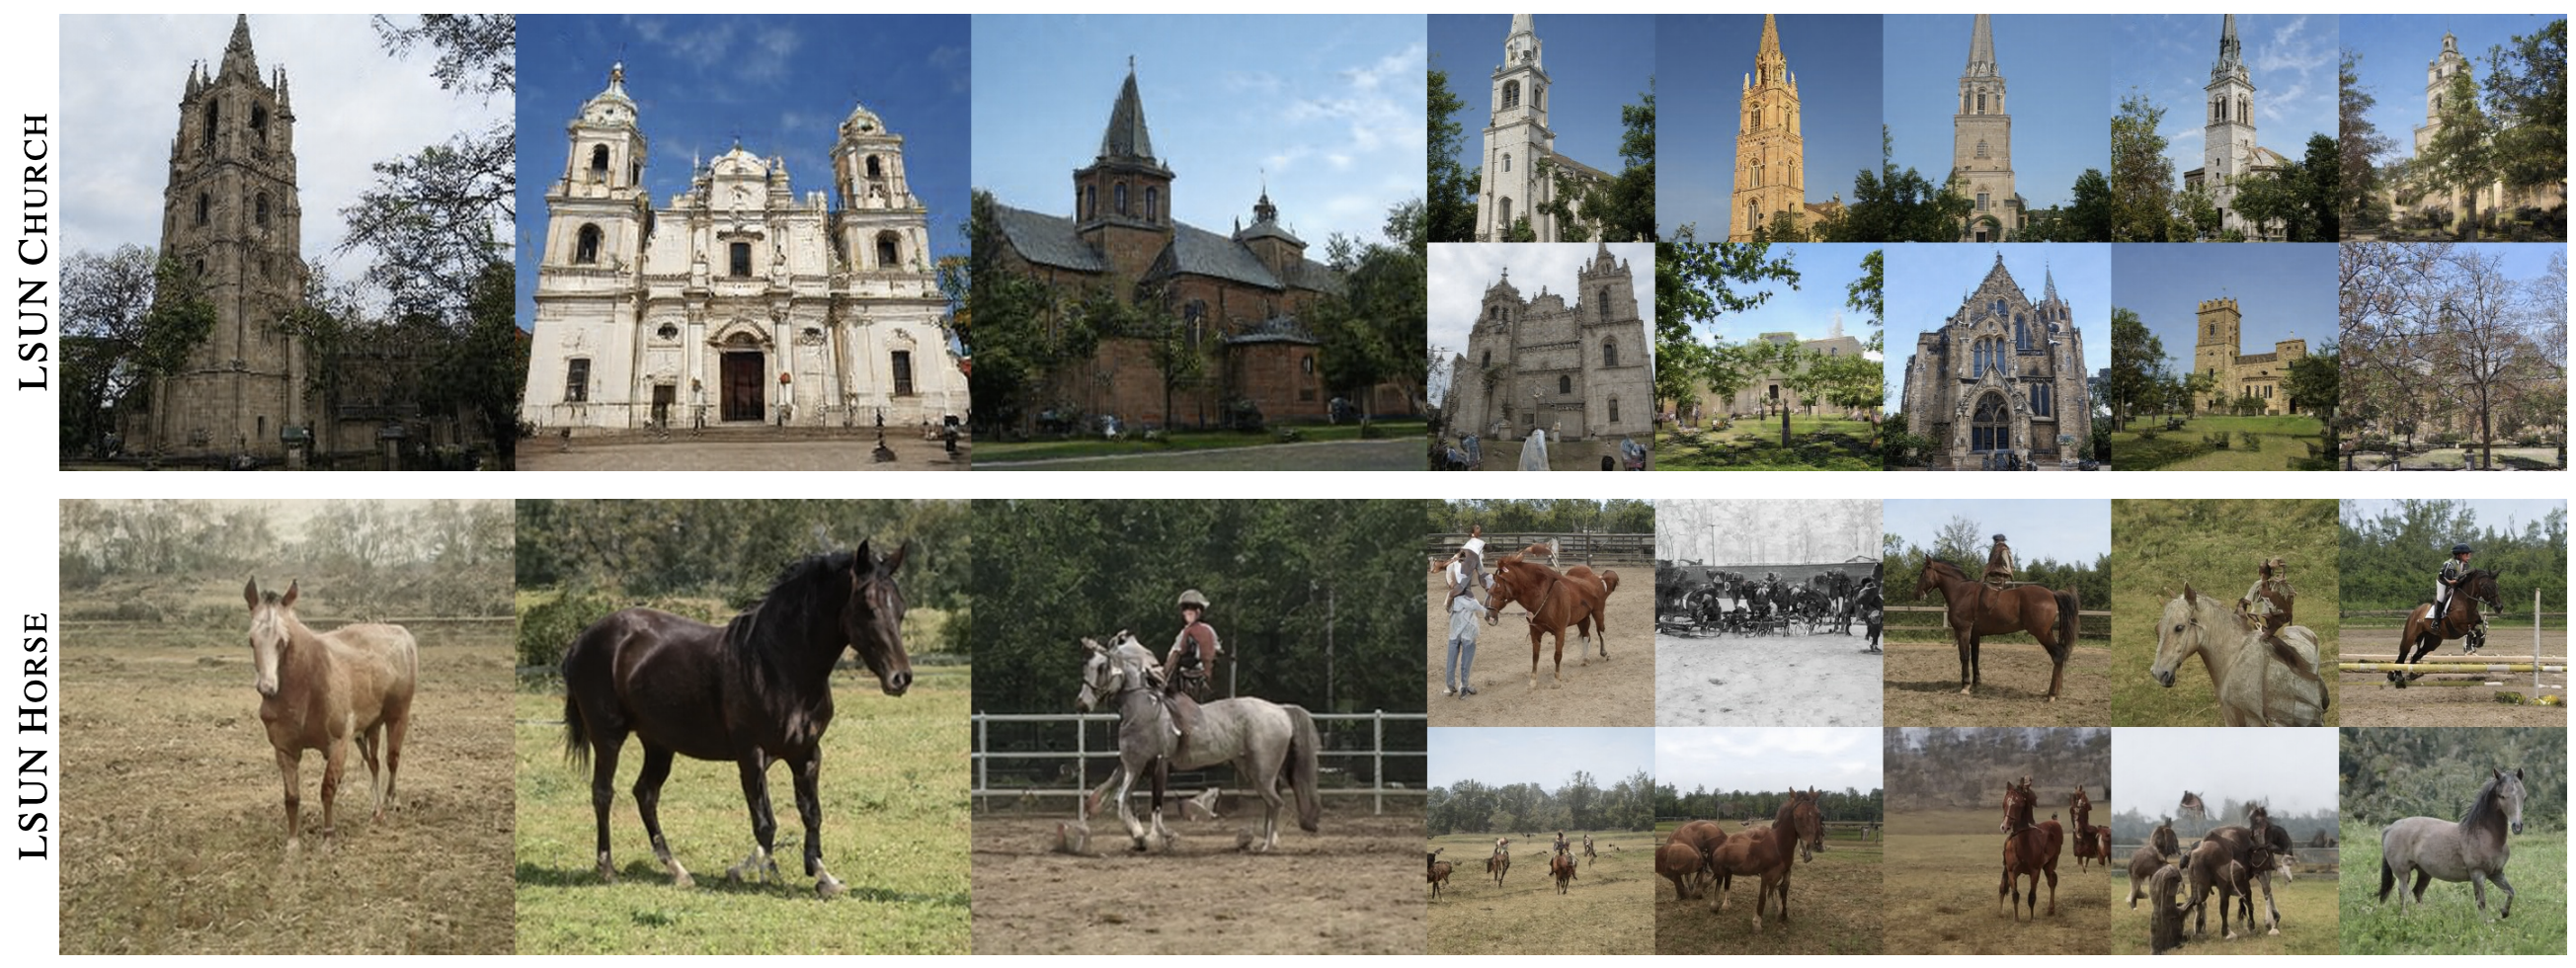
\includegraphics[width=\textwidth]{images/stylegan2-samples-2}
\end{figure}
\end{frame}


\begin{frame}{Final thoughts}
\begin{itemize}
    \item\pause Strong SotA for image generation
    \item\pause The ablation study is good
    \item\pause A lot of interesting gritty details are being discussed
    \item\pause They also observed a good improvement in quality by simply increasing a model size
    \item\pause They spent 51 GPU-years (v100-like) for the entire project
    \begin{itemize}
        \item\pause If it took 3 months, then it was equivalent to a \textit{constant} usage of 204 GPUs
    \end{itemize}
\end{itemize}
\end{frame}


\end{document}
